\chapter{Implementierung}
\label{implementierung}
In diesem Kapitel werden wichtige Aspekte bei der Implementierung des Systems aufgezeigt. Auf essentielle Quelltextausschnitte, welche für eine Gewährleistung, der aus den Anforderungen resultierenden Funktionalität verantwortlich sind, wird detailliert eingegangen. Dabei werden wichtige Konzepte, Strukturen und Designentscheidungen der entwickelten Architektur hervorgehoben und aufgetretene Probleme beim Implementierungsprozess dargelegt. Außerdem werden ausgewählte Subsysteme von \texttt{SimpliFX} mit geeigneten Darstellungsmitteln präsentiert und, für ein besseres Verständnis der zusammenarbeitenden Komponenten, eine beispielhafte Nutzung dieser durchgeführt. Die Verwendung und das Zusammenspiel der zuvor in \autoref{annotations} definierten Annotationen, werden durch Quelltextbeispiele erklärt. Dazu werden mögliche mit einhergehende Restriktionen beleuchtet.
\section{Architektur und Struktur der Software}
\label{architektur}
Für die Implementierung und um eine, nach \autoref{nreq3} und \autoref{nreq4}, hohe Softwarequalität sowie Erweiterbarkeit, muss das System durch eine wohlüberlegte Architektur repräsentiert werden. Um eine hohe Unabhängigkeit des Systems zu gewährleisten und eine Überladung mit unnötigen Funktion zu vermeiden, wurde auf die Nutzung von externen Bibliotheken zur Vereinfachung des Implementierungsprozesses und die Reduktion des Zeitaufwandes weitgehend verzichtet. Nur externe Bibliotheken, welche komplexe Funktionen zur Verfügung stellen und daher nicht im Rahmen dieser Arbeit implementiert werden können, sind im Projekt enthalten. Auch dürfen Bibliotheken, welche eine Inkompatibilität mit der im Projekt genutzten Softwarelizenz aufweisen, nicht als Abhängigkeit genutzt werden. Für die Verwaltung der externen Bibliotheken und die Strukturierung des Systems wird, wie in \autoref{konzept_und_modellierung_designentscheidungen} erläutert, das Apache Maven\footref{ft:maven} Build-Management-Tool verwendet. Das Projekt wird nach der finalisierten Implementierung als Maven-Artefakt öffentlich zugänglich und aufgrund der quelloffenen Natur auch per GitHub einsehbar sein. \texttt{SimpliFX} bietet dem Nutzer dazu auch verschiedene spezialisierte Artefakte an, welche an ein bestimmtes Framework für die Abhängigkeitsinjektion angepasst wurde. Für die interne Trennung der Belange und Funktionen von \texttt{SimpliFX}, werden Java Pakete verwendet. Diese Paketstruktur wird im nachfolgenden Unterkapitel näher erläutert. Dabei wird auf die Funktionalität der, in den einzelnen Paketen definierten, Klassen eingegangen und mögliche wichtige Funktionen, Methoden und Klassen mit Beispielen und ausgewählten Quelltextausschnitten vorgestellt und explizit angegeben, ob eventuelle Restriktionen bei der Nutzung zu beachten sind.
\section{Paketstrukturierung nach Funktionalität}
Die verschiedenen Pakete von \texttt{SimpliFX} sind in \autoref{fig:package_structure} dargestellt. Rot markierte Pakete dienen zur Abhängigkeitsinjektion und sind nicht im normalen Funktionsumfang enthalten, sondern nur mittels spezialisierter Maven Artefakte nutzbar. 
\def\Size{4pt}
\definecolor{folderbackground}{RGB}{135,147,154}
\tikzset{
  folder/.pic={
    \filldraw[draw=folderbackground,top color=folderbackground!50,bottom color=folderbackground]
      (-1.05*\Size,0.2\Size+5pt) rectangle ++(.75*\Size,-0.2\Size-5pt);  
    \filldraw[draw=folderbackground,top color=folderbackground!50,bottom color=folderbackground]
      (-1.15*\Size,-0.7*\Size) rectangle (1.15*\Size,\Size);
  },
  folderopt/.pic={
    \filldraw[draw=red,top color=red!50,bottom color=red]
      (-1.05*\Size,0.2\Size+5pt) rectangle ++(.75*\Size,-0.2\Size-5pt);  
    \filldraw[draw=red,top color=red!50,bottom color=red]
      (-1.15*\Size,-0.7*\Size) rectangle (1.15*\Size,\Size);
  }
}
\begin{figure}[H]
	\centering
	\begin{forest}
		for tree={
			font=\ttfamily,
			grow'=0,
			child anchor=west,
			parent anchor=south,
			anchor=west,
			inner xsep=8pt,
			inner ysep=0pt,
			if n=6{edge path={\noexpand\path [draw, \forestoption{edge}] (!u.south west)+(12.5pt,0) |- (.child anchor) pic {folderopt}\forestoption{edge label};}}{if n={12}{edge path={\noexpand\path [draw, \forestoption{edge}] (!u.south west)+(12.5pt,0) |- (.child anchor) pic {folderopt}\forestoption{edge label};}}{if n={15}{edge path={\noexpand\path [draw, \forestoption{edge}] (!u.south west)+(12.5pt,0) |- (.child anchor) pic {folderopt}\forestoption{edge label};}}{edge path={\noexpand\path [draw, \forestoption{edge}] (!u.south west)+(12.5pt,0) |- (.child anchor) pic {folder}\forestoption{edge label};}}}},
			if n children=0{}{
				delay={
					prepend={[,phantom, calign with current]}
				}
			},
			fit=band,
			before computing xy={l=35pt}
		}
		[de.intelligence.bachelorarbeit.simplifx
			[application]
			[classpath]
			[controller]
			[css]
			[dagger1]
			[di]
			[event]
			[events]
			[exception]
			[fxml]
			[guice]
			[localization]
			[shared]
			[spring]
			[utils]
		]
	\end{forest}
	\caption{Paketstruktur -- \texttt{SimpliFX}}
	\label{fig:package_structure}
\end{figure}
\subsection{Paket: utils}
Das \texttt{utils} Paket beinhaltet Klassen und Methoden, welche häufig genutzte Operationen an zentraler Stelle kombiniert. Außerdem werden Werkzeugklassen bereitgestellt, die in der Form nicht im Funktionsumfang von Java enthalten sind. Dazu gehören beispielsweise funktionale Schnittstellen mit einer Unterstützung von Ausnahmen, Klassen für das Überprüfen von Nullbarkeit oder bool'schen Bedingungen und Implementierungen der \texttt{Iterator} Schnittstelle, welche durch das Nutzen von \texttt{AutoCloseable}, Ressourcen schließen kann und damit eine Prävention von eventuellen Ressourcenlecks gewährleistet. Die Klasse \texttt{CloseableWrappedIterator}, erlaubt das Erstellen einer \texttt{Iterator} Instanz, welche bei Nutzung der \texttt{stream} Methode, alle genutzten Ressourcen bei einem Ende des Streams automatisch schließt. Außerdem wurde die Funktionalität der \texttt{Map.Entry} Klasse in die \texttt{Pair} Klasse ausgelagert, von welcher eine beispielhafte Nutzung in \autoref{lst:pair} dargestellt ist.
\begin{figure}[H]
	\begin{lstlisting}[caption=Beispiel -- Nutzung der \texttt{Pair} Klasse., captionpos=b, label=lst:pair]
final Pair<String, Integer> pair = Pair.of("test", 0);
System.out.println(pair.getLeft()); // test
System.out.println(pair.getRight()); // 0
	\end{lstlisting}
\end{figure}
\subsection{Paket: di}
\label{package_di}
Schnittstellen für die Unterstützung von Abhängigkeitsinjektion, werden durch das \texttt{di} Paket bereitgestellt. Die eigentliche Implementierung dieser Schnittstellen, ist in externen  Artefakten zu finden, auf welche in den folgenden drei Untersektionen näher eingegangen wird.
Das Paket stellt zwei Klassen, \texttt{DIEnvironment} und \texttt{IDIEnvironmentFactory} sowie die \texttt{@DIAnnotation} zur Verfügung. Wenn eine weitere Bibliothek zur Laufzeitinjektion von Abhängigkeiten genutzt werden soll, welche nicht im Funktionsumfang von \texttt{SimpliFX} enthalten sind, müssen Implementationen für beide Schnittstellen, sowie eine Annotation für die jeweilige Bibliothek bereitgestellt werden.
\begin{figure}[H]
	\centering
	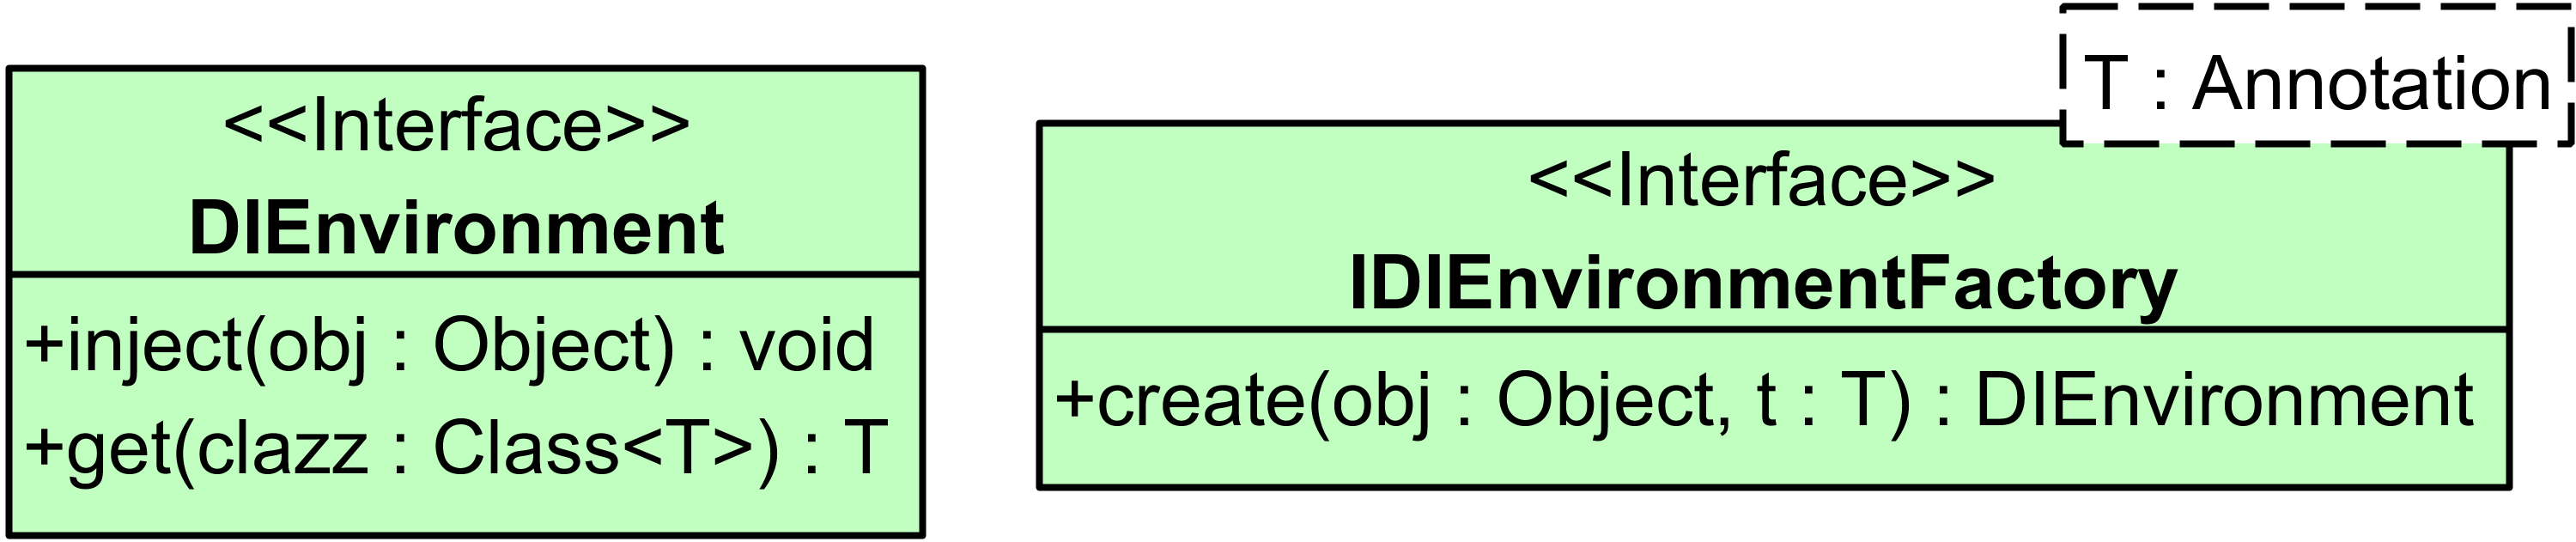
\includegraphics[width=\textwidth-2cm]{Abbildungen/DI Paket.png}
	\caption{Diagramm -- DI Schnittstellen.}
	\label{fig:di_package}
\end{figure}
\noindent \texttt{SimpliFX} kennt die Implementierung der in \autoref{fig:di_package} dargestellten Klassen nicht und kann daher mit Leichtigkeit um weitere Bibliotheken zur Abhängigkeitsinjektion erweitert werden. Zuerst muss der Entwickler eine Implementierung der \texttt{DIEnvironment} Klasse erstellen, welche für das Injizieren von vorhandenen Objekten und das Instanziieren von neuen Objekten verantwortlich ist. Danach muss eine \texttt{IDIEnvironmentFactory} mit dem Typen der Annotation als generischen Parameter erstellt werden, welche den alleinigen Zweck hat, neue Instanzen der vorher erstellten \texttt{DIEnvironment} Implementierung zu generieren. Letztlich muss der Entwickler eine Laufzeitannotation erstellen, welche an Typdefinitionen angebracht werden kann und dazu die Meta-Annotation \texttt{@DIAnnotation} mit der jeweiligen Implementierungsklasse der \texttt{IDIEnvironmentFactory} Schnittstelle als Parameter aufweist. Das Registrieren einer neuen Bibliothek ist in \autoref{appendix:add_new_di_library} gezeigt.
\subsection{Paket: dagger1}
Das \texttt{dagger1} Paket ist für die Integration von Dagger 1\footnote{Dagger 2 realisiert Abhängigkeitsinjektion ausschließlich zur Kompilierzeit, weshalb Schnittstellen zum reflektiven injizieren von Abhängigkeiten wie den \texttt{ObjectGraph} nicht mehr existieren und somit ein Zugang von \texttt{SimpliFX} auf den Injizierungsprozess ausgeschlossen ist.} in \texttt{SimpliFX} zuständig. Die \texttt{Dagger1Environment} Klasse definiert eine neue \texttt{ObjectGraph} Instanz aus den übergebenen Modulobjekten, welche für die Injektion verantwortlich ist. Dabei kann die Methode \texttt{ObjectGraph\#inject} genutzt werden, um Abhängigkeiten in eine vorhandene Instanz zu injizieren und \texttt{ObjectGraph\#get} um eine neue Klasseninstanz zu erstellen. 
\subsection{Paket: guice}
Das \texttt{guice} Paket ist für die Integration von Guice in \texttt{SimpliFX} zuständig. Dabei wird von der \texttt{GuiceEnvironment} Klasse ein neuer \texttt{Injector} erstellt, welcher durch die Methode \texttt{Injector\#injectMembers} Abhängigkeiten injiziert und mit \texttt{Injector\#getInstance} neue Instanzen erstellt.
\subsection{Paket: spring}
Das \texttt{spring} Paket ist für die Integration von Spring in \texttt{SimpliFX} zuständig.
Die Umgebungsklasse für Spring (\texttt{SpringEnvironment}) erstellt eine neue Instanz der \texttt{AnnotationConfigApplicationContext} Klasse, welche es ermöglicht, mittels einer \texttt{AutowireCapableBeanFactory}, Abhängigkeiten in bestehende Instanzen zu injizieren, sowie neue Instanzen aus Klassen zu erstellen.
\subsection{Paket: localization}
Alle Klassen und Funktionen, welche für das Umsetzen der dynamischen Lokalisierung benötigt wurden, sind im \texttt{localization} Paket enthalten. Dazu gehören beispielsweise die \texttt{II18N} Schnittstelle, eine Standard-Implementierung dieser und die \texttt{LocalizeValue} Annotation. 
\subsection{Paket: controller}
Das vollständige Controller-System ist im \texttt{controller} Paket enthalten. Das System kann auch unabhängig verwendet werden. Es ist jedoch ratsam, \texttt{SimpliFX} für die Initialisierung zu nutzen, da vorkonfigurierte Klassen wie beispielsweise \texttt{I18N} dafür benötigt werden. Das System kann durch die Erstellung eines neuen \texttt{IControllerGroup} Objektes gestartet werden. Die Schnittstelle stellt das Fundament des System dar und ist in \autoref{fig:controller_group_def} abgebildet. Durch die \texttt{start}-Methode kann die aktuelle Controllergruppe gestartet werden. Ist der Startcontroller zu dem Zeitpunkt noch nicht erstellt worden, so wird dieses mittels einem Aufruf der \texttt{constructController}-Methode nachgeholt. Diese Methode kann auch durch den Entwickler genutzt werden, um Controller zu generieren, bevor diese verwendet werden. Jede Gruppe muss exakt einen aktiven Controller besitzen, welcher durch \texttt{switchController} mit einer Standardanimation oder einer eigenen Animation gewechselt werden kann. Wird ein Controller bzw. eine Gruppe nicht weiter benötigt, so können mit den Aufruf der jeweiligen \texttt{destroy} Methode, alle gespeicherten Ressourcen und Instanzen gelöscht werden. Die von \texttt{SimpliFX} verwendete Implementierung dieser sowie eine Darstellung der verschiedenen Beziehungen zu anderen Komponenten des Systems ist in \autoref{appendix:controller_system} zu erkennen.
\begin{figure}[H]
	\centering
	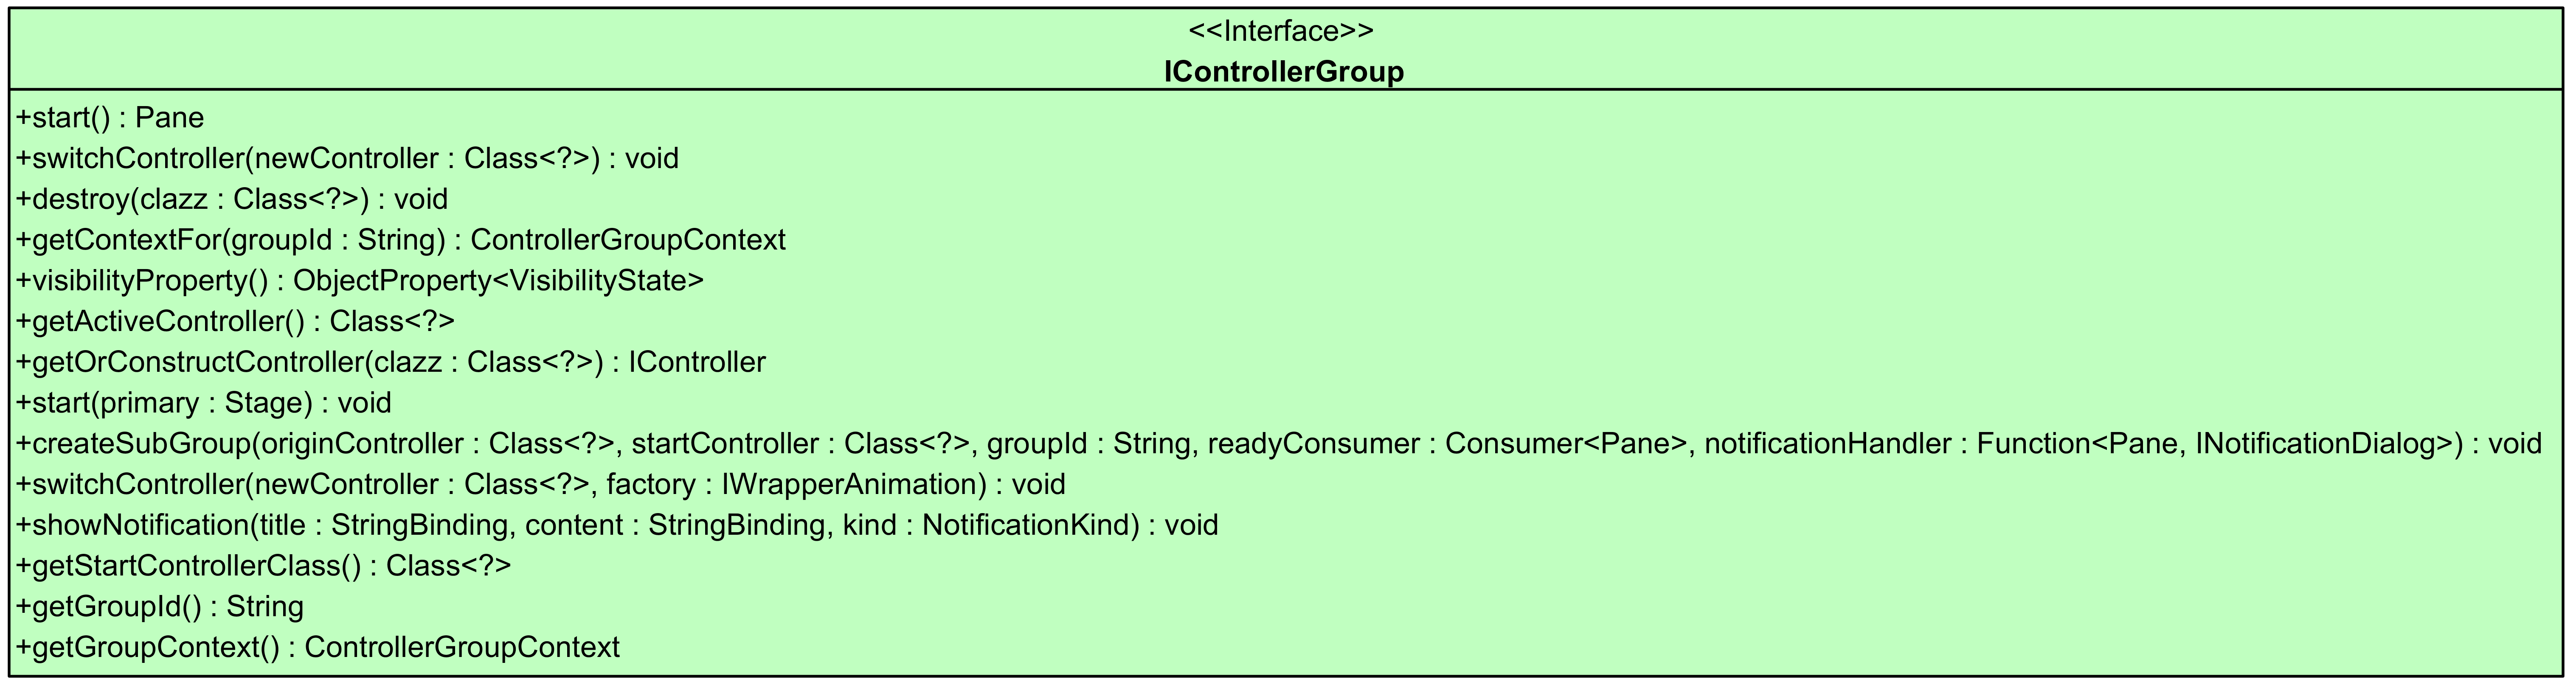
\includegraphics[width=\textwidth]{Abbildungen/Controller-System-Group.png}
	\caption{Diagramm -- Einstiegspunkt des Controller-Systems.}
	\label{fig:controller_group_def}
\end{figure}
Controllergruppen werden anhand eines \texttt{String}s eindeutig identifiziert und bei Konstruktion in einer globalen \texttt{ControllerRegistry} registriert, um doppelte Identifikatoren zu vermeiden. Dazu werden Controllerklassen vor der Konstruktion validiert, so ist es beispielsweise nicht erlaubt, eine nicht-statische, innere Klasse als Controller zu definieren, da eine direkte Instanziierung der Klasse durch \texttt{SimpliFX} in diesem Fall ausgeschlossen ist.
\subsection{Paket: exception}
Eigene Ausnahme-Klassen sind im \texttt{exception} Paket aufzufinden. Dazu gehören spezielle Ausnahmen für das Controller-System oder generelle Ausnahmen, welche von einer Vielzahl der \texttt{SimpliFX}-Komponenten genutzt werden.
\subsection{Paket: css}
Alle \ac{css} bezogenen Klassen sind im \texttt{css} Paket enthalten. Einige davon werden dabei ausschließlich durch den \texttt{SimpliFXMLLoader} genutzt um automatisch \ac{css} Metadaten für eigene JavaFX-Komponenten zu generieren. 
\subsection{Paket: classpath}
Wie bereits im Konzept beschrieben, wird für das Finden der Applikation- bzw. Preloader-Klasse ein System benötigt, welches in der Lage ist, den Klassenpfad zur Laufzeit des Programms nach Dateien zu durchsuchen. Dieses System findet nahezu alle Klassen und Ressourcen aus dem Klassenpfad, wird momentan aber nur für das Finden der jeweiligen Einstiegspunkte verwendet. Nur Klassenpfade aus einer unkomprimierten Orderstruktur (beispielsweise bei der Nutzung von verschiedenen Entwicklungsumgebungen) und aus komprimierten JAR-Archiven sind möglich. Die Architektur ermöglicht aber ein Hinzufügen von weiteren Klassenpfadquellen wie z.B. WAR-Archiven (siehe \autoref{fig:classpath_sources}). 
\begin{figure}[H]
	\centering
	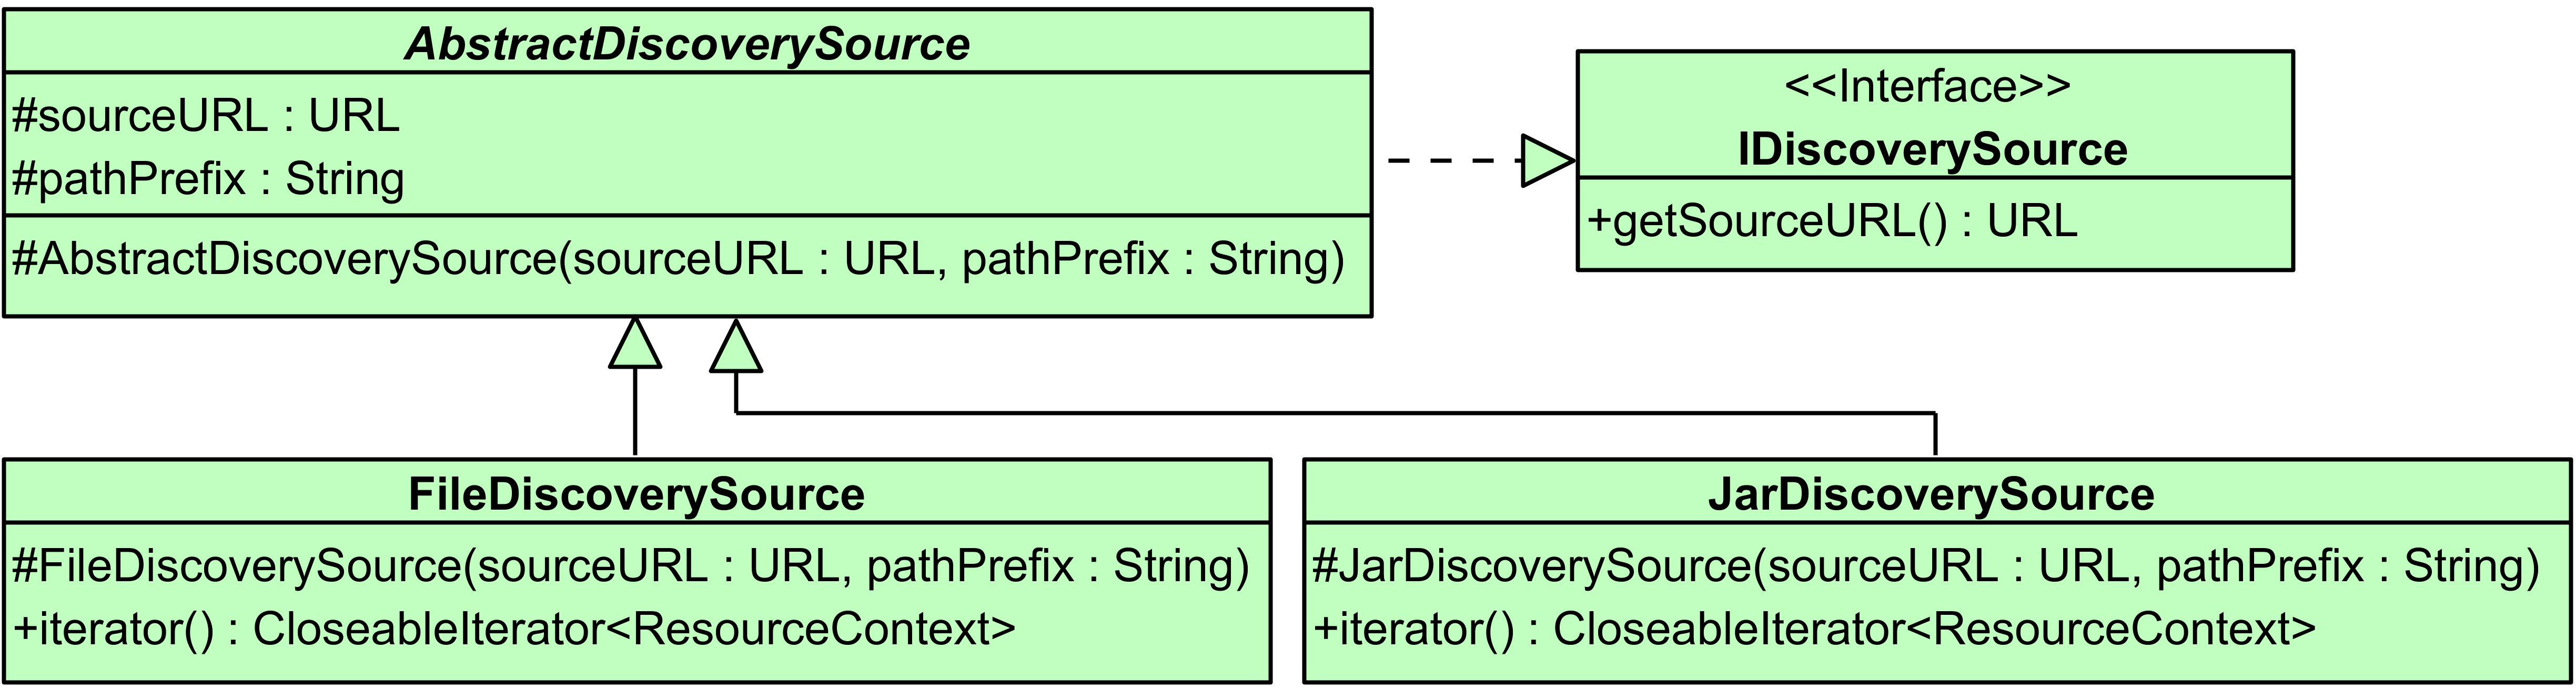
\includegraphics[width=\textwidth-2cm]{Abbildungen/Klassenpfadscan-Sources.png}
	\caption{Diagramm -- Mögliche Quellen für Klassenpfade.}
	\label{fig:classpath_sources}
\end{figure}
\noindent Damit ein Klassenpfadscan initiiert werden kann, muss, wie in \autoref{fig:classpath_interface} dargestellt, eine neue Instanz der \texttt{ClassDiscovery} Klasse erstellt werden. Eventuelle Konfigurationen wie das Hinzufügen weiterer \texttt{ClassLoader} oder dem Spezifizieren eines Basispfades, welcher den zu scannenden Klassenpfad einschränkt und somit in den meisten Fällen zu einer Reduktion der benötigten Scanzeit beiträgt, können durch die Nutzung des \texttt{DiscoveryContextBuilder} erreicht werden. Der \texttt{DiscoveryContextBuilder} bietet dabei auch standardisierte Konfigurationen an.
\begin{figure}[H]
	\centering
	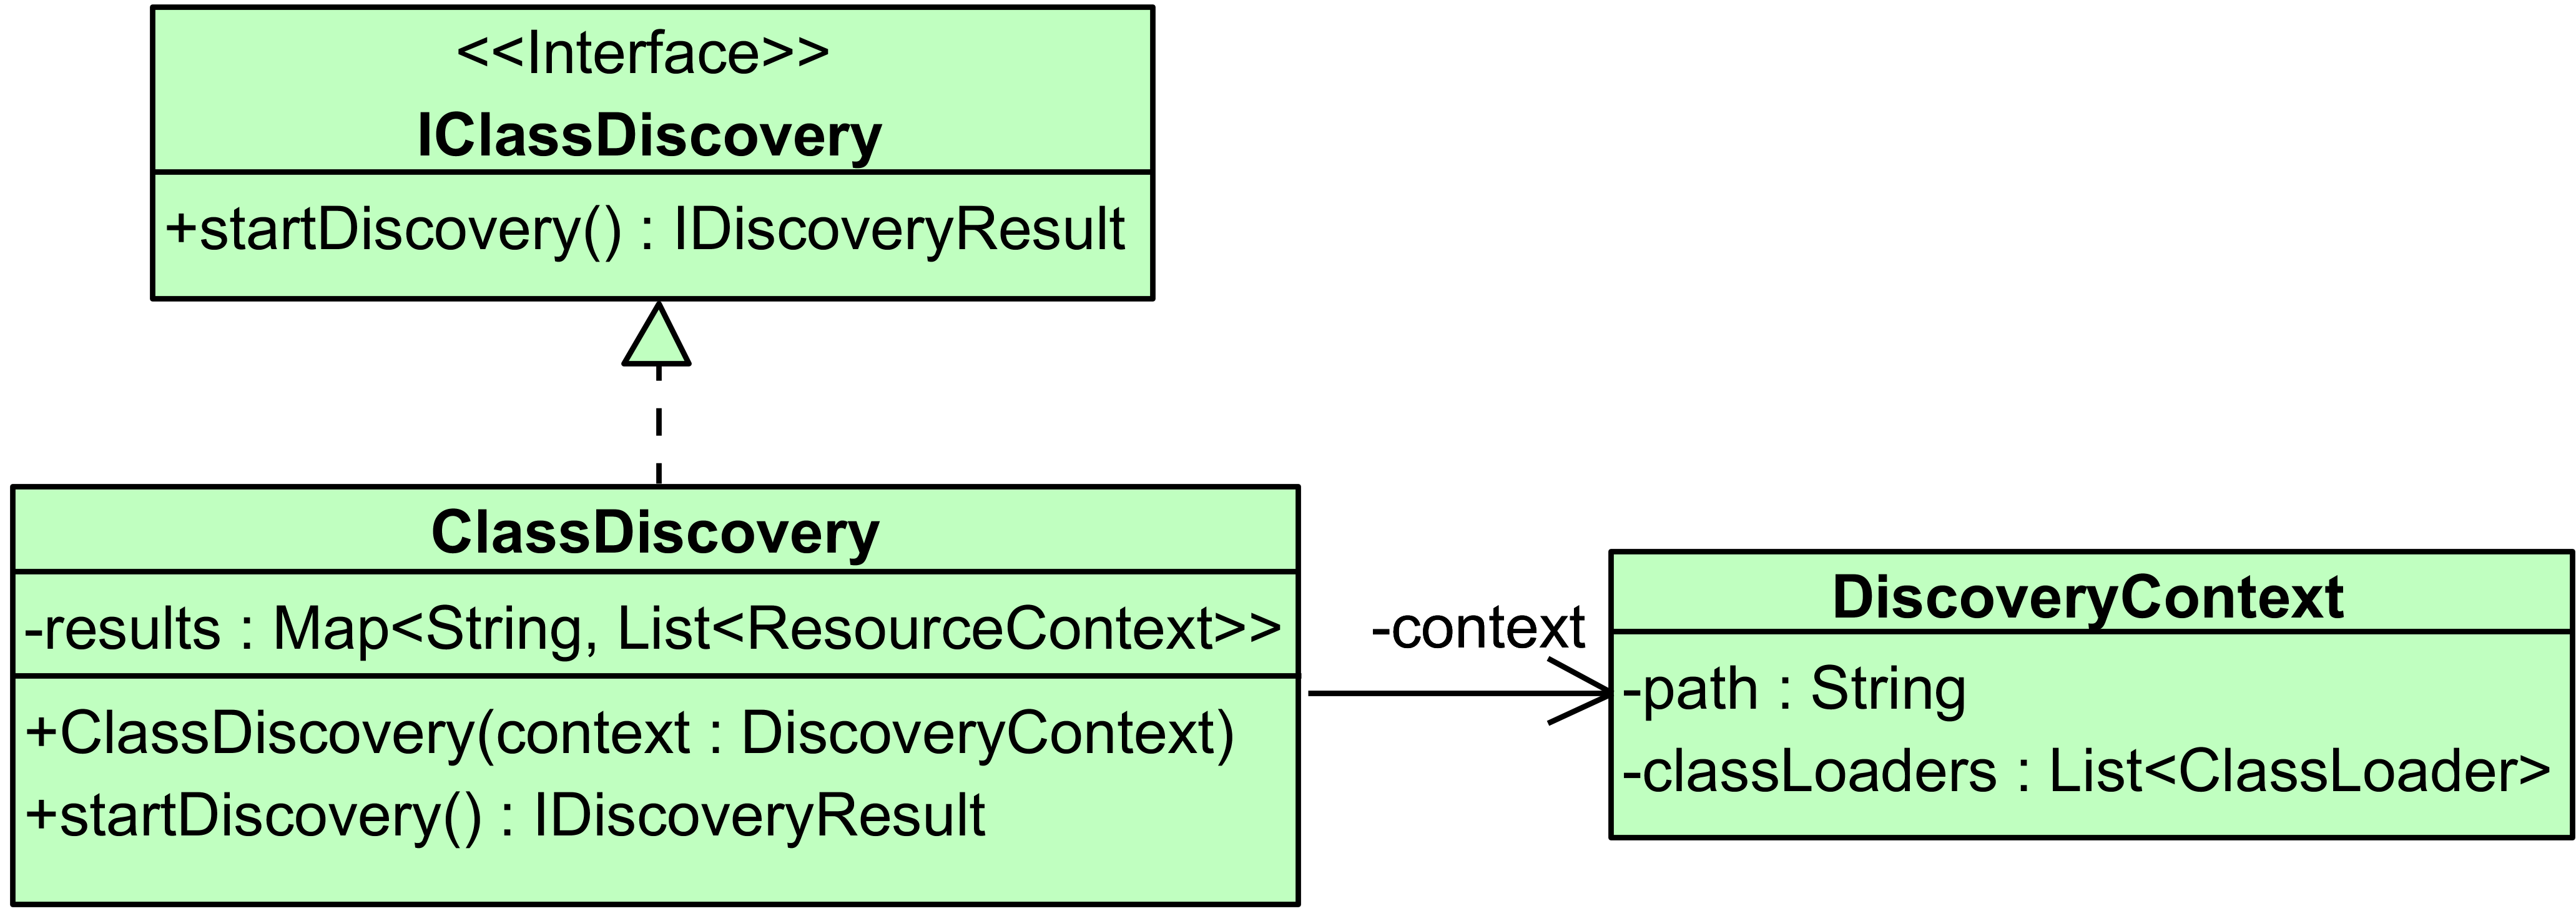
\includegraphics[width=\textwidth-2cm]{Abbildungen/Klassenpfadscan-Discovery.png}
	\caption{Diagramm -- Klassenpfad Schnittstelle und Implementierung.}
	\label{fig:classpath_interface}
\end{figure}
\noindent Eine beispielhafte Nutzung des Klassenpfadscans ist im folgenden Quelltextausschnitt dargestellt:
\begin{figure}[H]
	\begin{lstlisting}[caption=Beispiel -- Initiierung eines Klassenpfadscans., captionpos=b, label=lst:classpath_scan_usage]
// Startet einen Scan mit Standardkonfiguration
var r = new ClassDiscovery(new DiscoveryContextBuilder()
		.setDefaultClassLoaders().build()).startDiscovery());
// Sucht alle mit @StageConfig annotierten Klassen
List<Class<?>> a = r.findClassesAnnotatedBy(StageConfig.class);
	\end{lstlisting}
\end{figure}
\subsection{Paket: shared}
Die für das Konzept der geteilten Ressourcen benötigten Klassen wie zum Beispiel der \texttt{SharedResources} Klasse, welche alle globalen Ressourcen an zentraler Stelle sammelt und dem Entwickler bei Bedarf zur Verfügung stellt oder der \texttt{SharedFieldInjector} Klasse, welche für das Injizieren der Ressourcen in die Applikation sowie in alle neu erstellten Controller verantwortlich ist.
\subsection{Paket: event}
Das Event System findet seinen Ursprung im \texttt{event} Paket. Es setzt sich aus einer Schnittstelle, deren Implementierung und der \texttt{@EventHandler} Annotation zusammen. Die \texttt{IEventEmitter} Klasse (siehe \autoref{fig:event_emitter}) ermöglicht das Registrieren sowie das Abmelden eines Objektes beim System. Bei der Registrierung wird das übergebene Objekt auf Methoden untersucht, welche mit \texttt{@EventHandler} annotiert wurden, validiert diese und speichert sie in einem internen Methoden Cache. Die Validierung ist nötig, da gefundene Methoden nur exakt einen Parameter als Event aufweisen dürfen. 
\begin{figure}[H]
	\centering
	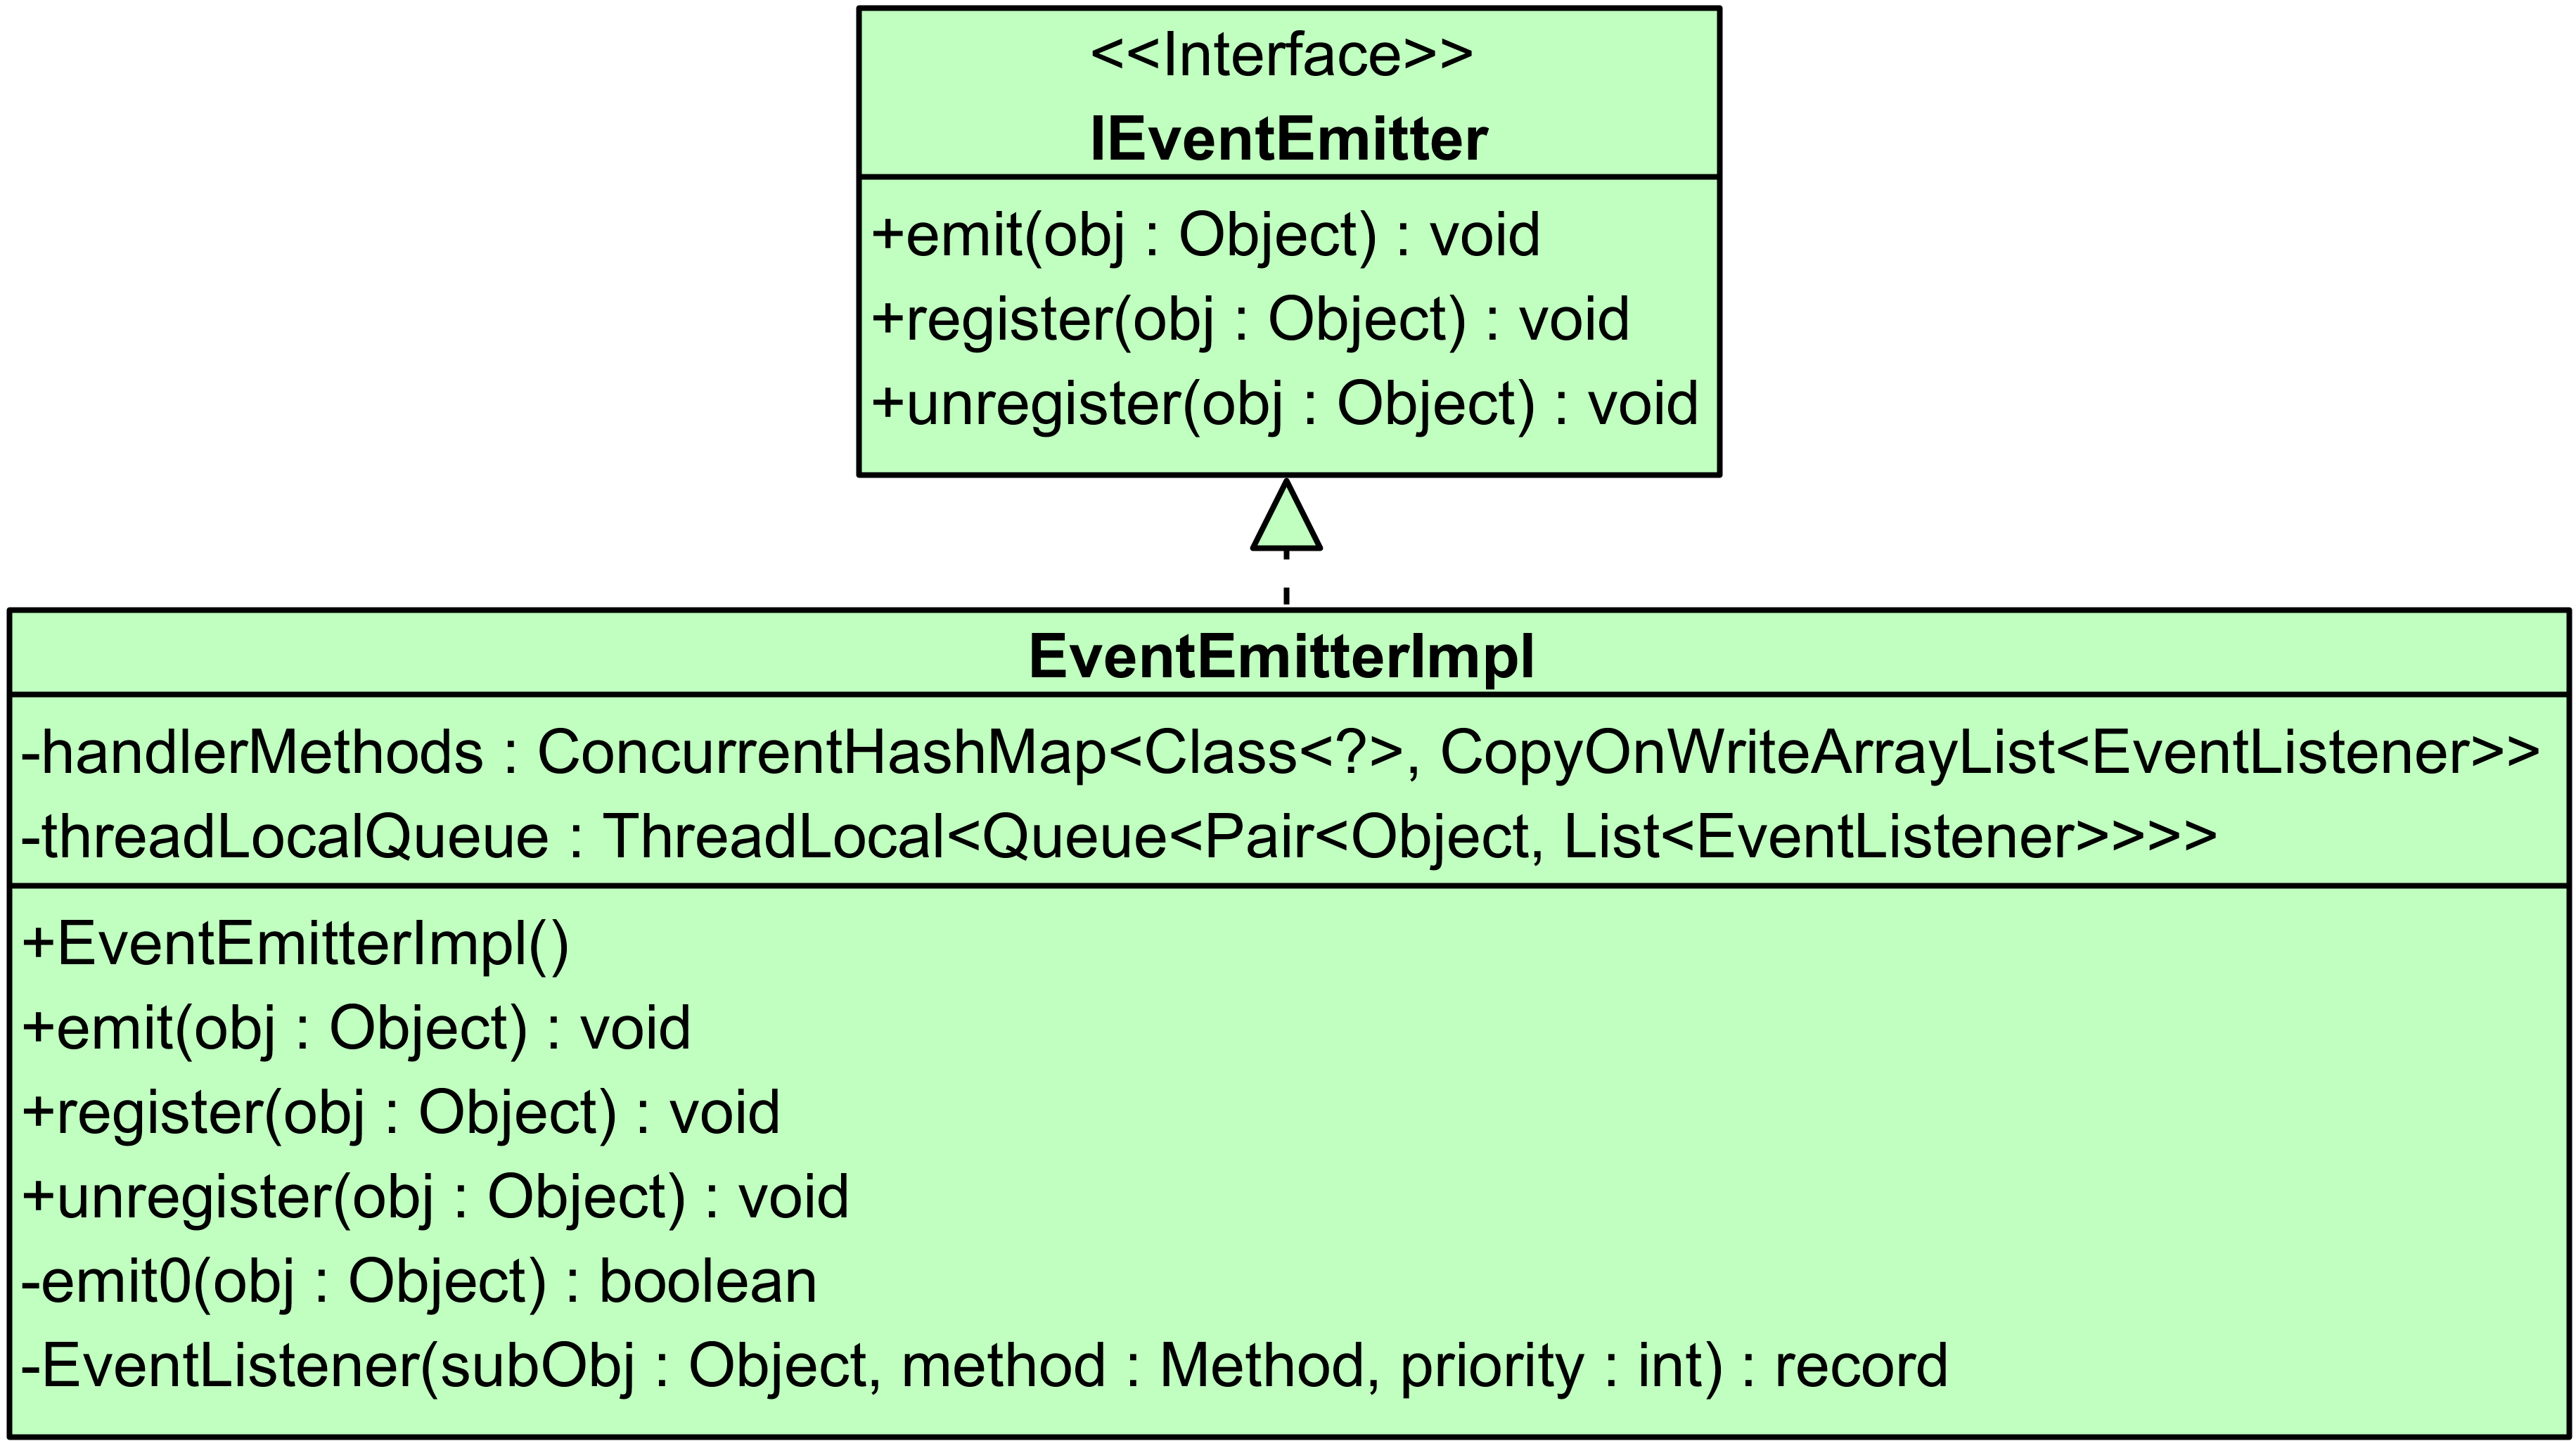
\includegraphics[width=\textwidth-4cm]{Abbildungen/EventEmitter.png}
	\caption{Diagramm -- IEventEmitter Schnittstelle und Implementierung.}
	\label{fig:event_emitter}
\end{figure}
\noindent Mit der \texttt{IEventEmitter\#emit} Methode, wird dem System ein neues Event übermittelt und alle Methoden welche für dieses Event registriert wurden, nach Priorität der Annotation aufgerufen. Die daraus resultierenden Methodenaufrufe werden dabei auf dem aufrufenden \texttt{Thread} ausgeführt und blockieren diesen, bis alle Aufrufe abgeschlossen wurden.
\subsection{Paket: events}
Das \texttt{events} Paket stellt eine Vielzahl an Standard-Events für beispielsweise den Lebenszyklus der Applikation (\texttt{InitEvent}, \texttt{StartEvent}, \texttt{StopEvent}) oder für Statusaktualisierungen des Preloaders (\texttt{StateChangeEvent}, \texttt{ProgressEvent}) bereit. Diese können durch eine \texttt{IEventEmitter} genutzt werden.
\subsection{Paket: application}
Die von \texttt{SimpliFX} verwalteten JavaFX Applikation- und Preloader-Klassen sowie die dafür benötigten Annotation sind im \texttt{application} Paket enthalten und definieren alle Methoden, welche durch die Applikation- respektive Preloaderklasse vererbt werden (siehe \autoref{fig:app_package}). Dabei wird bei der Erstellung der Klassen, eine für den Typ des Einstiegspunktes spezifische \texttt{IEventEmitter} Instanz übergeben, welche etwaige interne Methodenaufrufe in Form von vordefinierten Events an den vom Entwickler definierten, Einstiegspunkt delegiert.
\begin{figure}[H]
	\centering
	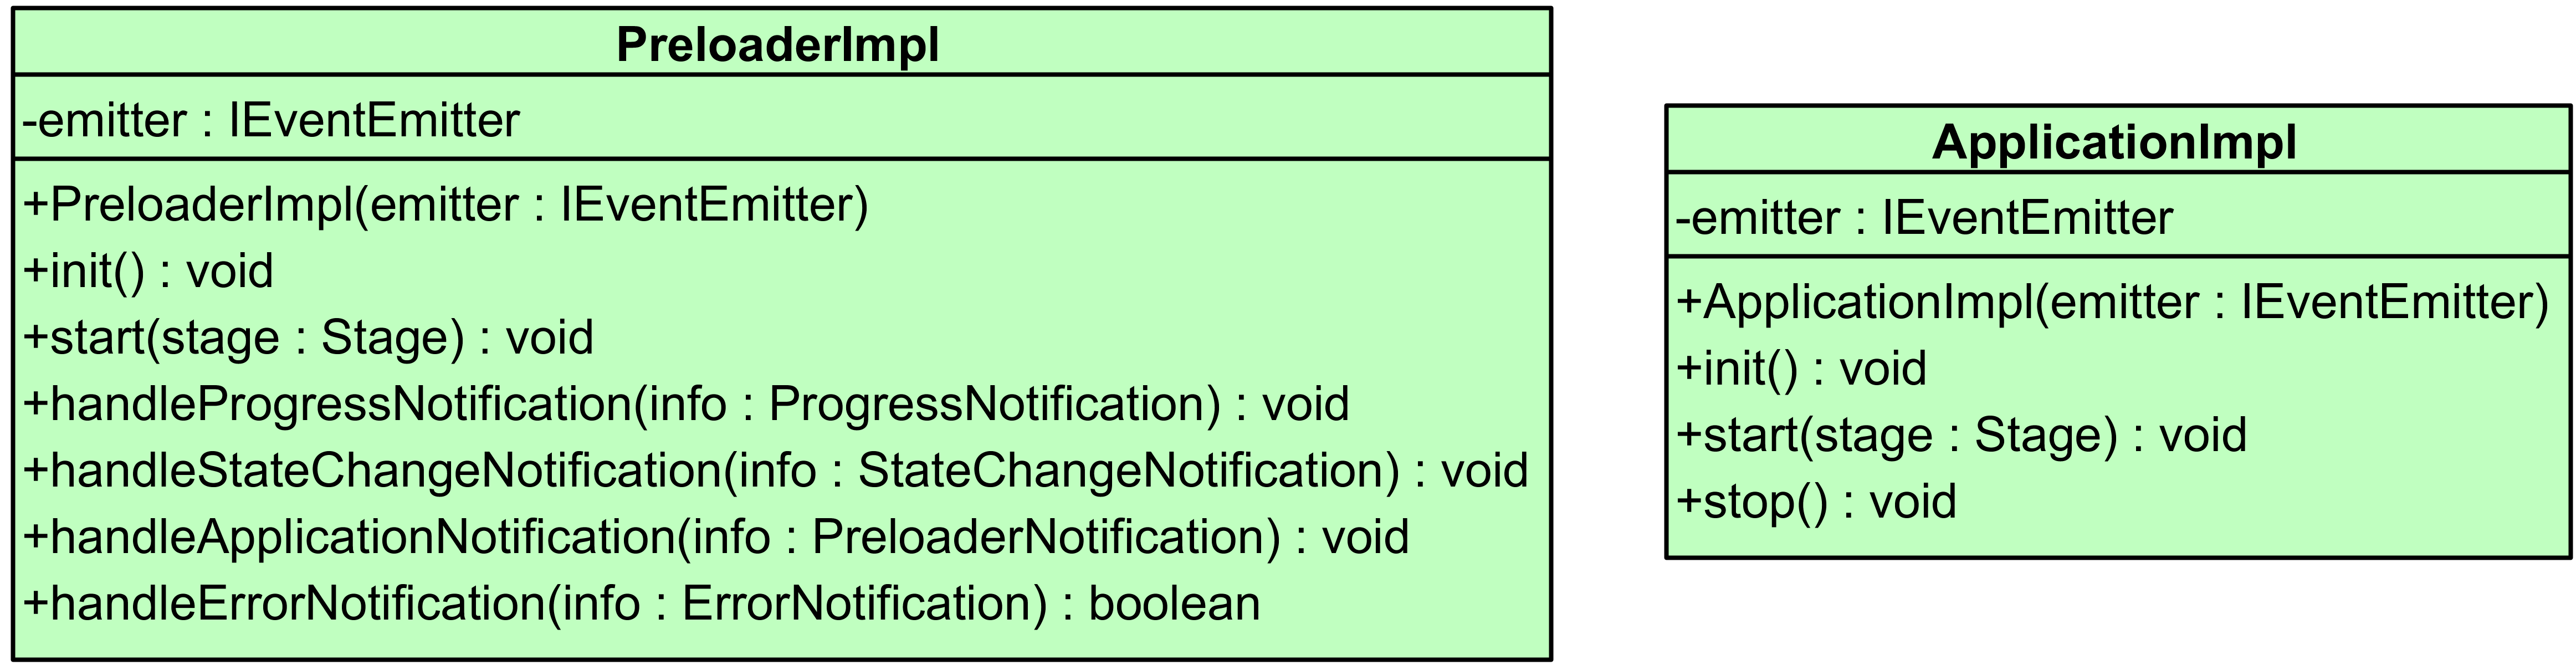
\includegraphics[width=\textwidth-2cm]{Abbildungen/Applikation und Preloader.png}
	\caption{Diagramm -- Applikation und Preloader.}
	\label{fig:app_package}
\end{figure}
\section{Essentielle Quelltextausschnitte}
In den folgenden Unterkapiteln werden wichtige Quelltextausschnitte, welche für Basisfunktionen von \texttt{SimpliFX} verantwortlich sind dargestellt und näher erklärt.
\subsection{SimpliFXMLLoader}
Der \texttt{SimpliFXMLLoader} unterstützt dieselbe XML-Syntax wie der \texttt{FXMLLoader}. Der einzige Unterschied liegt in der Verwendung von Übersetzungsschlüsseln aus Übersetzungsdateien. Das eigentliche Präfix zur Übersetzung (\glqq\texttt{\%}\grqq) wird automatisch durch den Loader in ein dynamisches Binding konvertiert. Ist die ursprüngliche Funktionalität der Übersetzung für bestimmte Elemente in der FXML Datei gewünscht, so kann das Präfix mit dem Voranstellen eines \glqq\texttt{!}\grqq{} erweitert werden. Der \texttt{SimpliFXMLLoader} unterstützt keine direkte Angabe von \texttt{ResourceBundle} Instanzen in den \texttt{load} Methoden oder den Konstruktoren. Stattdessen kann eine \texttt{II18N} Instanz übergeben werden. Um eine dynamische Übersetzung zu ermöglichen, musste das Behandeln von gefundenen Übersetzungsschlüsseln teilweise neu implementiert werden. Dazu wurde unter anderem die Methode (Zeilen 430--437) \texttt{Element\#resolvePrefixedValue} abgeändert. Ein einfaches Nutzen der \texttt{ResourceBundle\#getString} Methode ist für die gewünschte Dynamik ausgeschlossen. Stattdessen wurde eine neue innere Klasse definiert, welche das jeweils erstellte \texttt{StringBinding}, sowie den eigentlichen Übersetzungsschlüssel kapselt und Methoden zur Generation von parametrisierten Schlüsseln zur Verfügung stellt (\autoref{fig:translatable_property}). Die neue Implementierung der Ressourcenbehandlung ist in \autoref{lst:resource_handling} dargestellt.
\begin{figure}[H]
	\centering
	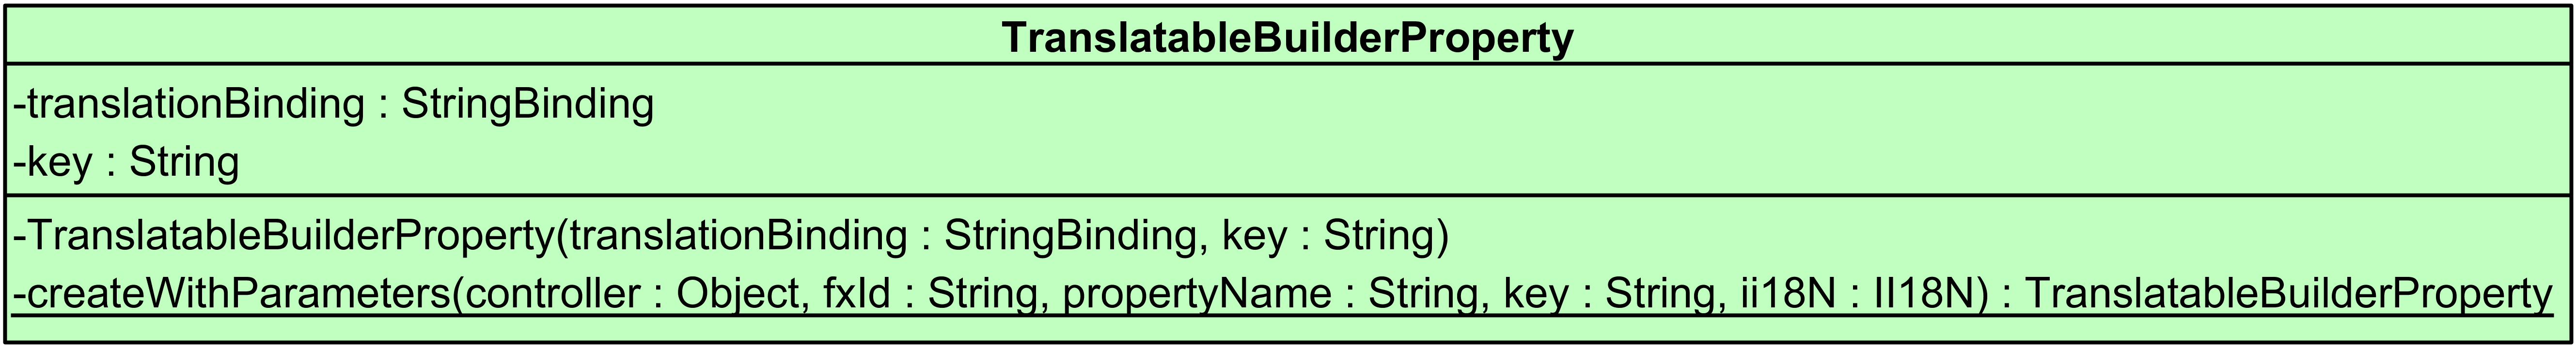
\includegraphics[width=\textwidth]{Abbildungen/Ressourcenbehandlung.png}
	\caption{Diagramm -- Klasse zur Datenkapselung von Übersetzungsinformationen.}
	\label{fig:translatable_property}
\end{figure}
\noindent Der Zugriff auf interne Properties von einfachen JavaFX-Komponenten wie zum Beispiel \texttt{Button} oder \texttt{Label} wird durch einen \texttt{BeanAdapter} ermöglicht, welcher automatisch durch den \texttt{FXMLLoader} erstellt wird. Mit diesem Adapter können Property-Felder auch nach Instanziierung der eigentlichen Komponentenklasse modifiziert und ausgelesen werden. Komplexe Komponenten wie \texttt{AreaChart}, werden mithilfe von \texttt{ProxyBuilder} Instanzen erstellt. Daraus resultiert, dass zum Zeitpunkt der Ressourcenbehandlung noch kein Objekt der Klasse instanziiert worden ist und trivialerweise kein Zugriff auf die internen Properties möglich ist. Aus dem Grunde, wird am Anfang der Behandlung überprüft, ob ein \texttt{BeanAdapter} für die aktuelle JavaFX-Komponente erstellt worden ist und anhand dessen das weitere Vorgehen bestimmt. Ist ein solcher Adapter präsent, kann ein \texttt{StringBinding} für die aktuelle Property aus der FXML Datei erstellt und bei vorhandenem Controller direkt mit eventuellen Parametern verknüpft werden. Andernfalls ist eine Erstellung eines \texttt{StringBinding}s für den Schlüssel an dieser Stelle nicht möglich. Für letztere Fälle wurden vereinzelte andere Quelltextabschnitte des Loaders modifiziert, auf welche hier aber nicht näher eingegangen wird.
\begin{figure}[H]
	\centering
	\begin{lstlisting}[caption=Implementierung -- Ressourcenbehandlung im \texttt{SimpliFXMLLoader}., captionpos=b, label=lst:resource_handling]
if (valueAdapter != null) {
	ObservableValue<?> val = valueAdapter.getPropertyModel("id");
	if (val instanceof StringProperty property && controller != null 
			&& propertyName != null) {
		return TranslatableBuilderProperty
				.createWithParameters(controller, property.get(), 
						propertyName, aValue, ii18N);
	}
	return new TranslatableBuilderProperty(ii18N
			.createBindingForKey(aValue), aValue);
} else {
	return new TranslatableBuilderProperty(null, aValue);
}
	\end{lstlisting}
\end{figure}
\subsection{Erweiterbare Abhängigkeitsinjektion}
Im Rahmen der Erweiterbarkeit (\autoref{TODO Erweiterbarkeit Anforderung NFA04}) wurde das System zur Abhängigkeitsinjektion weitgehend abstrakt gehalten. Wie in \autoref{package_di} erläutert und in \autoref{appendix:add_new_di_library} beispielhaft implementiert, ist es möglich neue Bibliotheken zur Laufzeitinjizierung hinzuzufügen, ohne dass \texttt{SimpliFX} Komponenten abgeändert werden müssen. Dazu werden alle Annotationen des Einstiegspunktes auf die Meta-Annotation \texttt{@DIAnnotation} überprüft. Ein exemplarischer Quelltextausschnitt, welcher dieses Konzept implementiert, ist in \autoref{lst:reflective_di} zu erkennen. Eine ähnliche Implementierung ist in \texttt{SimpliFX} verwendet worden.
\begin{figure}[H]
	\centering
	\begin{lstlisting}[caption=Implementierung -- Abhängigkeitsinjektion., captionpos=b, label=lst:reflective_di, basicstyle={\scriptsize\ttfamily}]
// Besitzt die Annotation die Meta-Annotation @DIAnnotation?
if (annotation.annotationType().isAnnotationPresent(DIAnnotation.class)) {
	// Finde IDIEnvironmentFactory Implementierung durch Annotationsparameter
	var factory = annotation.annotationType().getAnnotation(DIAnnotation.class)
			.value();
	// Starte Reflection-Prozess mit Factory als Einstiegspunkt
	ClassReflection classRef = Reflection.reflect(factory);
	// Finde Standardkonstruktor
	Optional<ConstructorReflection> constructorRefOpt = classRef.hasConstructor();
	if (constructorRefOpt.isEmpty()) {
		// Fehler - Kein Standardkonstruktor gefunden
		break;
	}
	// Erstelle neue Instanz der Factory
	IDIEnvironmentFactory<?> factoryInstance = constructorRefOpt.get()
			.instantiateUnsafeAndGet();
	// Finde einzige Methode der Factory
	MethodReflection methodRef = Reflection.reflect(factoryInstance)
			.reflectMethod("create", Object.class, 
					(Class<?>) ((ParameterizedType) factory.getGenericInterfaces()[0])
					.getActualTypeArguments()[0]);
	// Erstelle eine neue DIEnvironment Instanz
	SimpliFX.appDIEnv = methodRef.invokeUnsafe(applicationListener, annotation);
	break;
}
	\end{lstlisting}
\end{figure}